\documentclass[10pt]{beamer}
\usepackage{graphicx}
\usepackage{amsmath}
\usepackage{bm}
\usepackage{hyperref}
\usepackage{booktabs}
\usepackage{color}
\usepackage{xcolor}
\usepackage{amssymb}      % For \checkmark
\usepackage[utf8]{inputenc} % For ° and £ (or use \pounds)
\usepackage{tikz}
\usetikzlibrary{shapes.geometric, arrows, positioning, calc, fit, backgrounds}

% Enable speaker notes (uncomment one of these options)
%\setbeameroption{show notes} % Notes on separate pages
\setbeameroption{show notes on second screen=right} % Notes on second screen for presentation
\usepackage{pgfpages}

% TikZ styles for block diagrams
\tikzstyle{startstop} = [rectangle, rounded corners, minimum width=3cm, minimum height=1cm,text centered, draw=black, fill=red!30]
\tikzstyle{process} = [rectangle, minimum width=3cm, minimum height=1cm, text centered, text width=3cm, draw=black, fill=blue!20]
\tikzstyle{sensor} = [rectangle, minimum width=2.5cm, minimum height=0.8cm, text centered, text width=2.5cm, draw=black, fill=green!20]
\tikzstyle{power} = [rectangle, minimum width=2.5cm, minimum height=0.8cm, text centered, text width=2.5cm, draw=black, fill=yellow!30]
\tikzstyle{arrow} = [thick,->,>=stealth]

\usetheme{Boadilla}

\title{Free-Roving Subsea Cable Inspection Drone}
\subtitle{A Technical Feasibility Study}
\author{Jerry Liu (yhl63) \\ Zihe Liu (zl559)}
\institute{University of Cambridge}
\date{\today}

% Custom footnote settings
\setbeamercolor{footline}{use=structure,bg=structure.fg, fg=white}
\setbeamertemplate{footline}{%
  \leavevmode%
  \begin{beamercolorbox}[wd=\paperwidth,ht=2.5ex,dp=1ex]{footline}%
    \hfill
    \insertshorttitle
    \hfill
    \insertframenumber/\inserttotalframenumber
    \hspace{1em}
  \end{beamercolorbox}%
}

% Add section divider slides
\AtBeginSection{
  \begin{frame}
  \vfill
  \centering
  \begin{beamercolorbox}[sep=8pt,center,shadow=true,rounded=true]{title}
    \usebeamerfont{title}\insertsectionhead\par%
  \end{beamercolorbox}
  \vfill
  \end{frame}
}

\begin{document}

% Title slide
\frame{\titlepage}


%%%%%%%%%%%%%%%%%%%%%%%%%%%%%%%%%%%%%%%%%%%%%%%%%%%%%%%%%%%%%%%%%%%%%
\section{Problem - Subsea Cable Inspection}

\begin{frame}{Problem - Why Subsea Cables Matter}
  \begin{columns}[T]
    \begin{column}{0.45\textwidth}
      \textbf{Backbone of the Internet:}
      \begin{itemize}
        \item 97-99\% of intercontinental data traffic
        \item 500+ cables worldwide
        \item 14 million kilometers total
        \item 2-5 cm diameter (garden hose size)
      \end{itemize}
    \end{column}
    \begin{column}{0.52\textwidth}
      \includegraphics[width=\textwidth]{img/subsea\_cables.png}
    \end{column}
  \end{columns}

  \note{Before we dive into our design and feasibility assessment, let's give some context to the problem we're tackling: Subsea cables. Your internet connection, whether that be for online banking or video calls, 97-99\% of that data goes through a dense network of over 500+ undersea cables, spanning a total of 14 million kilometers over the seafloor making it THE largest and possibly greatest man-made infrastructure ever. This is the backbone of the internet, and when they fail, the consequences are severe. Despite the significance of these cables, these cables are no thicker than your average garden-hose around 2-5 cm in diameter, with hair-thin strands of optical fiber embedded within, designed to remain undisturbed across the seabed.}
\end{frame}

\begin{frame}{Problem - Current Limitations}
  \begin{columns}[T]
    \begin{column}{0.55\textwidth}
      \includegraphics[width=\textwidth]{img/ship.png}
    \end{column}
    \begin{column}{0.42\textwidth}
      \textbf{Cable Faults:}
      \begin{itemize}
        \item ~200 faults/year
        \item Shallow waters most vulnerable
        \item Shetland Islands 2022: 23,000 people offline
      \end{itemize}

      \vspace{0.5em}

      \textbf{Traditional: Tethered ROVs}
      \begin{itemize}
        \item[+] Unlimited power
        \item[+] Real-time comms
        \item[--] Limited range
        \item[--] Tether entanglement
        \item[--] High operational cost
      \end{itemize}
    \end{column}
  \end{columns}

  \vspace{1em}
  \centering
  \textit{Solution: Free-roving Autonomous Underwater Vehicle}

  \note{In shallow waters however, these subsea cables are susceptible to a wider range of disturbances, largely from human activities such as anchoring, or snagged by nets, resulting in roughly 200 faults a year. In October 2022, both cables serving the Shetland Islands were damaged. For days, 23,000 people had no internet, could not use card payments, could not access online banking. Businesses lost thousands. Emergency services were disrupted. These are not rare events, they require constant monitoring and effective maintenance. When a fault occurs, an army of ships strategically placed around the world would identify and repair the location of the fault, which usually involves the usage of a tethered drone to inspect the damaged cable. Despite the effectiveness of tethered communications and unlimited power, this comes at the cost of a limited range of motion and risks of entanglement, as well as higher maintenance costs for dedicated vessels. Therefore we propose the use of an untethered AUV}
\end{frame}


%%%%%%%%%%%%%%%%%%%%%%%%%%%%%%%%%%%%%%%%%%%%%%%%%%%%%%%%%%%%%%%%%%%%%
\section{Requirements and Operating Environment}

\begin{frame}{Requirements and Operating Environment}
  \textit{``A free-roving (no umbilical cable) submarine inspection drone is required for undersea cables: operating down to 250 m depth. It should have an endurance of 2 hours continuously powered operation, carrying video and ultrasound imaging equipment drawing a 30 W electrical load, and have suitable propulsion to travel up to 4 m/s peak speed with 1 m/s cruise. Total mass is to be $<$ 25 kg, to allow easy handling on board the mothership.''}

  \vspace{0.5em}

  \begin{columns}[T]
    \begin{column}{0.48\textwidth}
      \textbf{Key Specifications:}
      \begin{itemize}
        \item Depth: 250m (25 bar pressure)
        \item Endurance: 2 hours continuous
        \item Speed: 1 m/s cruise, 4 m/s peak
        \item Payload: 30W (imaging + ultrasound + lighting)
        \item Mass: $<$ 25 kg total
      \end{itemize}
    \end{column}

    \begin{column}{0.48\textwidth}
      \textbf{Operating Challenges:}
      \begin{itemize}
        \item Pressure: $P = \rho gh \approx 25$ bar
        \item Temperature: ~4°C seawater
        \item No GPS/RF underwater
        \item Saltwater corrosion
        \item Turbid water (limited visibility)
      \end{itemize}
    \end{column}
  \end{columns}

  \note{At 250 m depth, the pressure is approximately 25 bar (2.5 MPa). This is calculated using P = rho g h, where rho is seawater density (1027 kg/m cubed), g is gravitational acceleration, and h is depth. The temperature is approximately 4 degrees Celsius. Materials must resist corrosion - we will use 316 stainless steel and anodized aluminum. Sensors must work in turbid water with near-zero visibility. Communications are limited to acoustic modems underwater since radio and GPS signals cannot penetrate seawater beyond a few meters. The 30W payload limit includes all imaging equipment (camera), ultrasound sensors, and lighting - this is a combined budget, not separate allocations.}
\end{frame}


\begin{frame}{Problem Definition}
  \begin{columns}[T]
    \begin{column}{0.48\textwidth}
      \textbf{Hydrodynamics}

      Analyze underwater drag forces to estimate thrust needed for efficient movement.
      \begin{itemize}
        \item Degrees of freedom and stability control
        \item Drag and resistive forces
      \end{itemize}
    \end{column}

    \begin{column}{0.48\textwidth}
      \textbf{Mechanical Design}

      Develop the mechanical system ensuring all components fit within the 25kg weight limit.
      \begin{itemize}
        \item Buoyancy system
        \item Structural integrity
      \end{itemize}
    \end{column}
  \end{columns}

  \vspace{1em}

  \begin{columns}[T]
    \begin{column}{0.48\textwidth}
      \textbf{Power Consumption}

      Identify energy storage limits to define mission duration and vehicle size within constraints.
      \begin{itemize}
        \item 2 hours continuous operation
        \item Support 30W load as well as communications and mechanical systems
      \end{itemize}
    \end{column}

    \begin{column}{0.48\textwidth}
      \textbf{Communication and Control}

      Assess feasibility of underwater wireless communication methods for control and data transfer.
      \begin{itemize}
        \item Attenuation in seawater
        \item Navigation and mapping
      \end{itemize}
    \end{column}
  \end{columns}
\end{frame}

%%%%%%%%%%%%%%%%%%%%%%%%%%%%%%%%%%%%%%%%%%%%%%%%%%%%%%%%%%%%%%%%%%%%%
\section{Existing Commercial Solutions}

\begin{frame}{Existing Commercial Solutions}
  \begin{table}
    \scriptsize
    \begin{tabular}{lcccccc}
      \toprule
      \textbf{Model}      & \textbf{Type} & \textbf{Mass} & \textbf{Depth} & \textbf{Speed} & \textbf{Endurance} & \textbf{Cost} \\
      \midrule
      \textbf{Our Target} & AUV           & $<$25 kg      & 250m           & 4 m/s peak     & 2 hrs              & \$9-10K       \\
      \midrule
      Iver3 (L3Harris)    & AUV           & 27-39 kg      & 100m           & 1.3 m/s        & 8-14 hrs           & \$75-120K     \\
      ecoSUB m-Power+     & AUV           & 17 kg         & 500m           & ~1.5 m/s       & 8-10 hrs           & £35-50K       \\
      Boxfish AUV         & AUV           & 25 kg         & 300-600m       & ~2 m/s         & 10 hrs             & \$80-150K     \\
      BlueROV2            & ROV           & 10-11 kg      & 100-300m       & 1 m/s          & 3-5 hrs            & \$3-3.5K      \\
      \bottomrule
    \end{tabular}
  \end{table}

  \vspace{0.3em}

  \begin{columns}[T]
    \begin{column}{0.24\textwidth}
      \centering
      \includegraphics[width=0.9\textwidth]{img/iver3.png}
      \tiny Iver3: Single thruster + fins
    \end{column}
    \begin{column}{0.24\textwidth}
      \centering
      \includegraphics[width=0.9\textwidth]{img/ecosub.png}
      \tiny ecoSUB: 500m rated, alkaline
    \end{column}
    \begin{column}{0.24\textwidth}
      \centering
      \includegraphics[width=0.9\textwidth]{img/boxfish.png}
      \tiny Boxfish: Tethered AUV, 6-DOF
    \end{column}
    \begin{column}{0.24\textwidth}
      \centering
      \includegraphics[width=0.9\textwidth]{img/bluerobtoicsROV2.png}
      \tiny BlueROV2: Tethered ROV, 6-DOF
    \end{column}
  \end{columns}

  \vspace{0.3em}
  \centering
  Key finding: No commercial AUV $<$25 kg achieves 4 m/s sustained speed

  \note{Many commercial solutions exist but vary in capability. Commercial designs such as the Iver3 and ecoSUB use fully autonomous operation with single thruster plus fins for pitch/yaw control. The Boxfish uses 8 vectored thrusters for full 6-DOF control including hovering. BlueROV2 is included as it is a Blue Robotics reference platform that proves component viability, though it is a tethered ROV not an autonomous AUV. Key finding: Few commercial AUVs under 25 kg achieve 4 m/s sustained speed - most operate at 1.5-2.5 m/s due to power limitations. Commercial pricing (50-150K dollars) reflects support and warranty, not just hardware costs. Our target specifications are ambitious but achievable with careful trade-off management.}
\end{frame}

%%%%%%%%%%%%%%%%%%%%%%%%%%%%%%%%%%%%%%%%%%%%%%%%%%%%%%%%%%%%%%%%%%%%%
\section{Design Approach and System Architecture}

\begin{frame}{Trade-offs}
  \begin{center}
    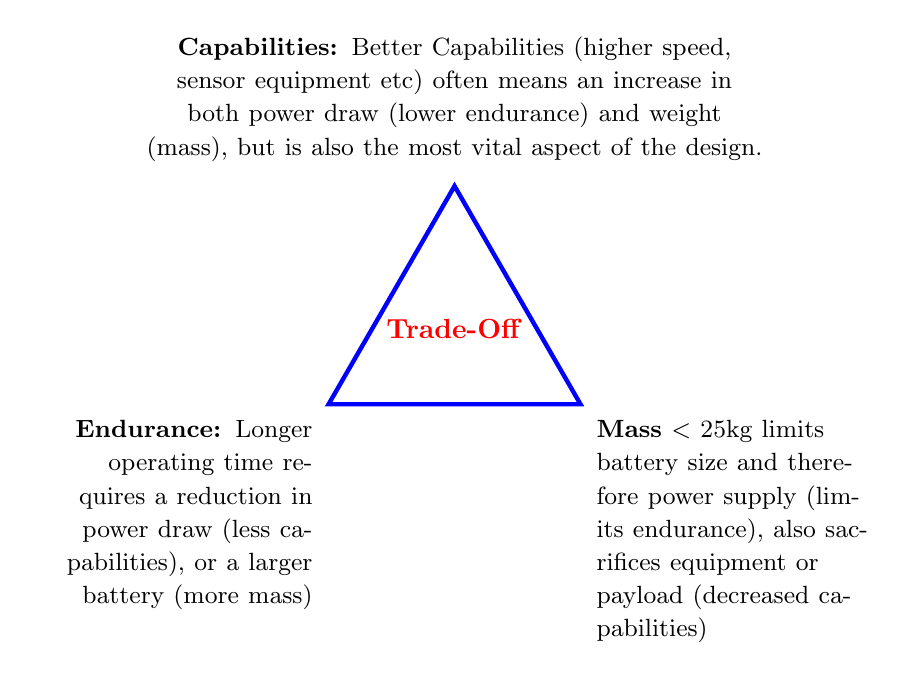
\begin{tikzpicture}[scale=0.8]
      % Triangle
      \draw[ultra thick, blue] (0,0) -- (4,0) -- (2,3.464) -- cycle;

      % Center text
      \node[text width=2.5cm, align=center] at (2,1.2) {
        \textcolor{red}{\textbf{Trade-Off}}
      };

      % CAPABILITIES (top vertex)
      \node[text width=8cm, align=center, anchor=south] at (2,3.7) {
        \small \textbf{Capabilities:} Better Capabilities (higher speed, sensor equipment etc) often means an increase in both power draw (lower endurance) and weight (mass), but is also the most vital aspect of the design.
      };

      % ENDURANCE (bottom left vertex)
      \node[text width=3.5cm, align=right, anchor=north east] at (-0.1,-0.1) {
        \small \textbf{Endurance:} Longer operating time requires a reduction in power draw (less capabilities), or a larger battery (more mass)
      };

      % MASS (bottom right vertex)
      \node[text width=3.5cm, align=left, anchor=north west] at (4.1,-0.1) {
        \small \textbf{Mass} $<$ 25kg limits battery size and therefore power supply (limits endurance), also sacrifices equipment or payload (decreased capabilities)
      };
    \end{tikzpicture}
  \end{center}

  \vspace{0.5em}
  \textbf{Our Solution:} \textit{Mission profile with 80\% cruise (1 m/s) + 20\% sprint (4 m/s)}

  \note{
    The design is constrained by three competing requirements forming a trade-off triangle. Capabilities - speed, sensors, and mission functionality - drive both power consumption and weight. Better capabilities mean higher speed requiring more thrust power, and more sensor equipment adding weight.

    Endurance requires either reducing power draw or installing larger batteries. Reducing power limits capabilities. Larger batteries add weight, conflicting with the mass constraint.

    Mass under 25 kilograms limits battery capacity to 4 to 5 kilograms maximum. This restricts available energy, which directly limits either endurance or capabilities.

    The solution is a mission profile approach: 80 percent time at 1 meter per second cruise speed, 20 percent time at 4 meters per second peak speed. Average power is much lower, which satisfies all three constraints simultaneously.
  }
\end{frame}


\begin{frame}{System Design Directions}
  \begin{center}
    \begin{itemize}
      \item Autonomous/programmable solution to remove the need for high-quality real-time data transmission which limits untethered ROVs
            \begin{itemize}
              \item Enables self-contained operation with onboard power, navigation, and data handling
              \item Supports scalable inspection missions without reliance on surface tethers
            \end{itemize}

      \item 4-thruster design gives a good balance between maneuverability, stability, and power efficiency
            \begin{itemize}
              \item Sufficient for precise hovering and pitch/yaw stability
              \item Redundancy for safe recovery in case of partial thruster failure
              \item Efficient low-speed maneuvering for inspection tasks
            \end{itemize}
      \item Hull design to be cylindrical (pill) shaped to minimise volume as well as simplify hydrodynamic calculations.
            \begin{itemize}
              \item Streamlined shape reduces drag forces at higher speeds
              \item Simplifies internal component layout and waterproofing
              \item Proven design in existing AUVs for balance of speed and stability
            \end{itemize}
    \end{itemize}
  \end{center}

  \note{
    The design uses an autonomous approach instead of untethered ROV operation, as untethered ROVs require continuous high-bandwidth communication for real-time control, which is only possible with a physical cable limiting range and adding complexity. Autonomous operation enables self-contained missions with onboard power, navigation, and data storage.

    The 4-thruster configuration provides full 6-degree-of-freedom control. Four horizontal thrusters control surge, sway, and yaw. Two vertical thrusters control heave, pitch, and roll. This enables precise hovering at fixed positions for detailed cable inspection, and lateral motion without changing heading. Redundancy allows safe recovery if one thruster fails. The configuration is efficient for low-speed maneuvering typical of inspection tasks.

    The cylindrical pill-shaped hull minimizes drag and simplifies hydrodynamics. At 4 meters per second, drag force is 0.5 times density times velocity squared times drag coefficient times frontal area. A streamlined torpedo shape achieves drag coefficient 0.28 to 0.32, significantly lower than spherical hulls at 0.47. The cylindrical geometry also simplifies internal component layout and pressure vessel calculations using standard ASME formulas.
  }
\end{frame}

\begin{frame}{System Architecture - Simplified Block Diagram}
  \begin{center}
    \centering
    \includegraphics[width=0.9\textwidth]{img/System\_design.png}
  \end{center}

  \vspace{0.5em}
  \centering
  \small Modular architecture enables phased development and testing

  \note{This simplified system architecture shows the five main subsystems. POWER provides 803 Wh from three 18Ah lithium-ion batteries at 14.8V. CONTROL uses the Navigator flight controller with dual IMUs plus Raspberry Pi 4 running ArduSub for mission control, along with depth sensor, compass, and surface GPS. PROPULSION consists of four T200 thrusters controlled by ESCs. PAYLOAD includes camera, Ping360 sonar, and lights totaling 30W. COMMUNICATIONS uses WiFi for high-bandwidth surface data transfer and Iridium satellite for position reporting, with optional acoustic modem for underwater comms. This modular design allows independent testing and phased development.}
\end{frame}

%%%%%%%%%%%%%%%%%%%%%%%%%%%%%%%%%%%%%%%%%%%%%%%%%%%%%%%%%%%%%%%%%%%%%


\section{Communications and Navigation}

\begin{frame}{Underwater Communication Challenges}
  \textbf{Underwater Communication:}
  \begin{itemize}
    \item High signal attenuation limits the usage of radio frequency signals - effective range only a few metres
    \item Optical communication limited by turbidity and scattering - short range, line-of-sight only
    \item Acoustic communication is the only viable option for long-range underwater comms, but inherently slow, high latency, and affected by multipath
  \end{itemize}

  \vspace{0.5em}

  \textbf{Result:} Minimise communication underwater — store data onboard, transfer at surface

  \note{
    Before diving into our design decisions, it’s important to understand why underwater communication and navigation are inherently difficult problems.

    First, radio waves — which power all our terrestrial wireless communication — are heavily absorbed by seawater. Even at low frequencies, the signal strength drops to unusable levels within just a few meters.

    Optical communication, like lasers or LEDs, can achieve higher data rates, but only in clear water and over short, line-of-sight distances — typically less than 100 meters.

    That leaves acoustics as the only practical long-range option. Acoustic modems can reach several kilometers, but at a steep cost: data rates of only a few kilobits per second, high latency, and unit prices easily exceeding twelve thousand dollars.

    For our small, autonomous inspection drone, these trade-offs simply aren’t efficient.

    As a result, our design minimizes underwater communication by storing all sensor data onboard during the mission and transferring it to the surface once the vehicle resurfaces. This approach maximizes data throughput while avoiding the complexities of underwater communication.

  }
\end{frame}

\begin{frame}{Communications Systems}
  \textbf{Multi-Mode Communication Strategy:}

  \begin{table}
    \footnotesize
    \begin{tabular}{llll}
      \toprule
      \textbf{Mode}         & \textbf{Product}         & \textbf{Specifications}      & \textbf{Cost}  \\
      \midrule
      \textbf{Surface WiFi} & \textbf{802.11n module}  & 2.4/5 GHz, 150 Mbps          & \textbf{\$50}  \\
                            & (Raspberry Pi built-in)  & 50-100m range in air         &                \\

      \midrule
      \textbf{Satellite}    & \textbf{RockBLOCK 9603N} & Iridium Short Burst Data     & \textbf{\$260} \\
                            &                          & 340 byte messages            &                \\
                            &                          & Global coverage (open ocean) &                \\
                            &                          & GPS position reporting       &                \\

      \bottomrule
    \end{tabular}
  \end{table}

  \vspace{0.5em}

  \textbf{Operational Modes:}
  \begin{itemize}
    \item \textbf{At surface:} WiFi for high-bandwidth video/data + GPS fix
    \item \textbf{Open ocean:} RockBLOCK for GPS position reporting every 10 min
  \end{itemize}

  \note{
    When the AUV surfaces, it uses the Raspberry Pi 4’s built-in WiFi with a marine-grade antenna to transfer data at around 150 megabits per second. This allows a complete upload of all mission data such as recorded video — roughly 7–8 gigabytes — in just a few minutes. Surfacing every 30 minutes lets us offload data incrementally when the vehicle is in the 50-100 meter range, reducing onboard storage requirements and ensuring data safety even if the vehicle is lost.

    For open-ocean or long-range missions, we include a RockBLOCK 9603N Iridium module. It provides global satellite coverage and transmits compact status messages — GPS coordinates, depth, and system health — every 10 minutes.  This ensures vehicle recoverability and global operational capability.

    Excluding acoustic and optical modems dramatically reduces costs, as acoustic systems cost over 12,000 dollars, have very low bandwidth (under 20 kbps), and are impractical for transferring gigabytes of data.
  }
\end{frame}

\begin{frame}{Navigation Scoping Calculations}

  \begin{itemize}
    \item MEMS IMUs measure angular rate and acceleration; position is estimated by integrating these signals.
    \item \textbf{Integration:} $\theta(t) = \int \omega \, dt$ (orientation); $\; x(t) = \iint a \, dt^2$ (position)
    \item Each integration amplifies sensor noise and bias:
    \item Without correction, small biases lead to large accumulated position errors over time.
  \end{itemize}

  \vspace{0.8em}

  \textbf{Drift Mitigation Strategies:}
  \begin{enumerate}
    \item \textbf{Zero-velocity updates:} Detect stationary periods and reset velocity estimates.
    \item \textbf{Sensor fusion:} Combine IMU with magnetometer and depth sensor for heading and vertical stabilization, or DVL to constrain horizontal drift.
    \item \textbf{Cable-relative navigation:} Use sonar or visual tracking to constrain lateral drift.
    \item \textbf{Surface GPS fix:} Acquire GPS position during surfacing to reset accumulated horizontal error.
  \end{enumerate}


  \note{
    \textbf{Speaker Notes:}

    When designing a free-roving underwater vehicle, one of the biggest challenges is maintaining a reliable sense of position and orientation without GPS.
    One of the most cost-effective solutions is to rely on an Inertial Measurement Unit, or IMU, which combines gyroscopes and accelerometers to track motion.
    However, IMU-based navigation underwater is an integration problem: we integrate angular rate for orientation and acceleration twice for position.
    This process inherently accumulates error—random noise grows as the square root of time, and bias causes linear drift.
    Over long missions, these effects can lead to significant position uncertainty if left uncorrected.

    Our mitigation strategy combines multiple complementary techniques:
    zero-velocity detection to reset errors during stationary periods,
    sensor fusion to stabilize heading and depth,
    cable-relative tracking using sonar or vision to maintain lateral alignment,
    and periodic GPS updates during surfacing to reset accumulated horizontal drift.

    Together, these methods ensure reliable navigation for cable inspection, with accuracy sufficient for operational needs without requiring costly DVL systems.
  }
\end{frame}

\begin{frame}{Navigation System Component Options}
  \textbf{Core Navigation Stack:}

  \begin{table}
    \scriptsize
    \begin{tabular}{lllll}
      \toprule
      \textbf{Component}         & \textbf{Specification} & \textbf{Performance}                   & \textbf{Cost} \\
      \midrule
      \textbf{Flight Controller} & Navigator (dual IMU)   & 2.8°/s/$\sqrt{\mathrm{Hz}}$ gyro noise & \$220         \\
                                 & Pixhawk 6C             & Similar performance                    & \$300         \\
      \midrule
      \textbf{Depth Sensor}      & Bar30 (MS5837)         & 2mm resolution, ±2m accuracy           & \$90          \\
                                 & Keller PA-7LD          & ±0.3m accuracy, stable                 & \$200-500     \\
      \midrule
      \textbf{Surface GPS}       & u-blox NEO-M8N         & 2.5m accuracy                          & \$35          \\
                                 & RTK GPS                & $<$0.1m accuracy                       & \$300-600     \\
      \midrule
      \textbf{Computer}          & Raspberry Pi 4         & Quad-core ARM, 4GB RAM                 & \$75          \\
      \midrule
      \textbf{DVL (Optional)}    & Nortek DVL1000         & 0.2 cm/s, <1m over 2 hrs               & \$20,000      \\
                                 & Teledyne Pathfinder    & Similar, proven                        & \$18-28K      \\
      \bottomrule
    \end{tabular}
  \end{table}


  \vspace{0.5em}

  \textbf{Baseline Cost: \$420} (Navigator + Bar30 + u-blox + RPi4)

  \note{
    Our navigation system is built around the Blue Robotics Navigator, which integrates dual IMUs and magnetometers for reliable attitude and heading estimation. It connects directly to the Raspberry Pi, reducing cabling and improving reliability. At 220 dollars, it costs 27 percent less than Pixhawk 6C (300 dollars) and is fully supported by ArduSub, a proven open-source autopilot.

    Depth is measured with the Bar30 pressure sensor, offering 2 mm resolution and 2 m accuracy, ideal for maintaining a 2–5 m altitude during cable inspection.

    At the surface, a u-blox NEO-M8N GPS resets accumulated IMU drift with ~2.5 m accuracy, which is sufficient for our 30-minute surface intervals—no need for costly RTK GPS.

    We also considered a DVL like the Nortek DVL1000 for sub-meter accuracy, but at  a 15–25k dollar price and +1.2 kg weight, it’s unnecessary for cable-following missions.

    Altogether, the baseline navigation stack — Navigator (220), Bar30 (90), GPS (35), and Raspberry Pi 4 (75) — costs 420 dollars total.
  }
\end{frame}



%%%%%%%%%%%%%%%%%%%%%%%%%%%%%%%%%%%%%%%%%%%%%%%%%%%%%%%%%%%%%%%%%%%%%
\section{Hydrodynamics and Propulsion Analysis}

\begin{frame}{Hydrodynamic Drag}
  \textbf{Vehicle Geometry (Torpedo Hull):}
  \begin{itemize}
    \item Diameter: $D = 0.3$ m, Length: $L = 1.2$ m
    \item Frontal area: $A = \frac{\pi D^2}{4} = 0.0707$ m$^2$
    \item Drag coefficient: $C_D = 0.28$--$0.32$ \protect\href{https://www.mdpi.com/2311-5521/6/7/252}{\textsuperscript{[MDPI CFD]}}
  \end{itemize}

  \vspace{0.5em}

  \textbf{Drag Force Equation:}
  $$F_D = \frac{1}{2} \rho v^2 C_D A$$

  Where $\rho = 1027$ kg/m$^3$ (seawater)

  \vspace{0.5em}

  \begin{itemize}
    \item \textbf{At 1 m/s cruise} $C_D = 0.32$: $F_D = 11.6$ N
    \item \textbf{At 4 m/s peak} $C_D = 0.28$: $F_D = 162$ N
  \end{itemize}

  \note{
    Hydrodynamic drag is the fundamental constraint on our design. The drag equation shows that drag force scales with velocity squared. Doubling speed quadruples drag force.

    Vehicle geometry is torpedo-shaped: 1.2 meters long, 0.3 meters diameter. The length-to-diameter ratio of 4 to 1 optimizes streamlining. Frontal area is 0.071 square meters.

    Drag coefficient C-D varies from 0.28 to 0.32 with speed. At low speeds, flow separation and turbulence near protrusions increases C-D to 0.32. At high speeds, Reynolds number increases, boundary layer becomes thinner, and C-D drops to 0.28. These values are validated against CFD studies on AUVs (MDPI 2021, DOI: 10.3390/jmse6070252).

    At 1 meter per second, drag is 11.6 newtons. At 4 meters per second, drag is 162 newtons - a 14-fold increase for 4-times speed increase. This quadratic relationship creates the fundamental challenge: high speed requires overcoming dramatically higher drag forces.
  }
\end{frame}

\begin{frame}{Power Requirements and Thruster Efficiency}
  \textbf{Mechanical power:} $P_{mech} = F_D \times v$

  \textbf{Electrical power:} $P_{elec} = \frac{P_{mech}}{\eta}$ (thruster efficiency $\eta \approx 0.55$ at high load\href{https://bluerobotics.com/store/thrusters/t200-thruster-r2-rp/}{\textsuperscript{[T200]}})

  \vspace{1em}

  \begin{table}
    \begin{tabular}{lccccc}
      \toprule
      \textbf{Speed} & $F_D$ (N) & $P_{mech}$ (W) & $\eta$                                                                                             & $P_{elec}$ (W) & \textbf{Notes}  \\
      \midrule
      1 m/s cruise   & 11.6      & 11.6           & 0.30\href{https://bluerobotics.com/store/thrusters/t200-thruster-r2-rp/}{\textsuperscript{[T200]}} & 39             & Low efficiency  \\
      4 m/s peak     & 162       & 648            & 0.55\href{https://bluerobotics.com/store/thrusters/t200-thruster-r2-rp/}{\textsuperscript{[T200]}} & 1,178          & High efficiency \\
      \bottomrule
    \end{tabular}
  \end{table}

  \vspace{0.5em}

  \textit{4 m/s requires 1.2 kW propulsion power (30× cruise power)}

  \note{
    Power scales with velocity cubed because power equals force times velocity. Drag force has v-squared, multiplied by another v from the power equation gives v-cubed scaling.

    Thruster efficiency varies with load. At 1 meter per second, mechanical power required is 11.6 watts, but thruster efficiency at light load is only 30 percent, requiring 39 watts electrical.

    At 4 meters per second, mechanical power is 648 watts - much higher than at cruise speed. At heavy load, thruster efficiency increases to 55 percent, so electrical power is 1,178 watts.

    The critical number: 1,178 watts propulsion at peak versus 39 watts at cruise. This is 30 times more power for 4 times speed. Pure v-cubed scaling would give 64 times, but efficiency improvement at high load reduces this to 30 times.

    This cubic scaling makes sustained high-speed underwater operation challenging. The constraint is battery energy, which translates directly to weight. Battery energy requirements conflict with the 25 kilogram mass limit.
  }
\end{frame}
\begin{frame}{Thruster Selection - T200}
  \begin{table}
    \scriptsize
    \setlength{\tabcolsep}{4pt}
    \begin{tabular}{lcccccc}
      \toprule
      \textbf{Model}  & \textbf{Thrust (N)} & \textbf{Power (W)} & \textbf{Depth (m)} & \textbf{Mass (kg)} & \textbf{Cost (\$)} & \textbf{Thrust/Cost} \\
      \midrule
      \textbf{T200}   & \textbf{51.5 fwd}   & \textbf{390 max}   & \textbf{300}       & \textbf{0.427}     & \textbf{230}       & \textbf{0.22}        \\
      SeaBotix BTD150 & 28                  & 80                 & 150                & 0.5                & 800                & 0.035                \\
      Maxon MT30      & 49                  & 180                & 6000               & 0.45               & 2,500              & 0.020                \\
      T500            & 158                 & 1000+              & 300                & 1.1                & 690                & 0.23                 \\
      \bottomrule
    \end{tabular}
  \end{table}

  \vspace{0.3em}

  \begin{columns}[T,onlytextwidth]
    \begin{column}{0.49\textwidth}
      \small
      \textbf{4× T200 Configuration:}
      \begin{itemize}
        \setlength{\itemsep}{0pt}
        \setlength{\parskip}{0pt}
        \item Total thrust: \textbf{206 N}
        \item Required: 162 N
        \item Propulsion cost: \$920
        \item ESCs (4× 30A): \$160
      \end{itemize}
    \end{column}

    \begin{column}{0.49\textwidth}
      \small
      \textbf{Justification:}
      \begin{itemize}
        \setlength{\itemsep}{0pt}
        \setlength{\parskip}{0pt}
        \item 6-20× lower cost than alternatives
        \item Adequate thrust
        \item 300m depth rating (vs 250m spec)
        \item Proven reliability
      \end{itemize}
    \end{column}
  \end{columns}

  \note{
    Four thruster options were evaluated. SeaBotix BTD150 has good efficiency but insufficient thrust: 28 newtons versus 51.5 newtons for T200. Maxon MT30 has 6000 meter depth rating and costs much more than T200 - unnecessary for 250 meter requirement. T500 provides 158 newtons thrust but draws over 1 kilowatt continuously and weighs 1.1 kilograms.

    T200 offers best thrust-to-cost ratio at 0.22 newtons per dollar. Four T200 thrusters provide 206 newtons total thrust for 162 newtons required - 27 percent safety margin. This margin accommodates deviation in drag coefficient calculations.

    We also need 4 Electronic Speed Controllers. We need one for each of the four thrusters. This is the small electronic board that takes the command from our flight controller and the power from the battery, and then precisely controls the motor's speed and direction.
  }
\end{frame}

%%%%%%%%%%%%%%%%%%%%%%%%%%%%%%%%%%%%%%%%%%%%%%%%%%%%%%%%%%%%%%%%%%%%%
\section{Power Budget and Energy Storage}

\begin{frame}{Complete System Power Budget}
  \begin{table}
    \footnotesize
    \begin{tabular}{lccc}
      \toprule
      \textbf{Subsystem}                   & \textbf{Cruise (W)} & \textbf{Peak (W)} & \textbf{Notes}   \\
      \midrule
      Propulsion (4× T200)                 & 39                  & 1,178             & Dominant at peak \\
      Payload (camera, lighting and sonar) & 30                  & 30                & Low-light USB    \\
      Navigation sensors                   & 5                   & 5                 & IMU, depth, GPS  \\
      Control (RPi4+Nav)                   & 10                  & 10                & ArduSub firmware \\
      Comms (WiFi/Iridium)                 & 2                   & 2                 & Surface only     \\
      \midrule
      \textbf{TOTAL}                       & \textbf{86 W}       & \textbf{1,225 W}  &                  \\
      \bottomrule
    \end{tabular}
  \end{table}

  \vspace{0.3em}

  \centering
  $P_{avg} = 314 \text{ W}$ (Accounting for mission profile)

  \note{
    The 30 watt payload specification is a combined budget for all payload components: camera at 2.5 watts, sonar at 2 to 5 watts, and lighting at 10 to 20 watts adjustable. Total payload is 15 to 28 watts, within the 30 watt limit.

    Propulsion dominates total power at peak speed: 1,225 watts total system power, with 1,178 watts for propulsion alone.

    The mission profile gives an average power of 314 watts: 0.8 times 86 plus 0.2 times 1,225. This average power determines battery capacity requirements.
  }
\end{frame}

\begin{frame}{Battery Sizing}
  \textbf{Energy Requirements:}
  $$E = P_{avg} \times t = 314 \text{ W} \times 2 \text{ h} = 628 \text{ Wh required}$$

  \begin{table}
    \scriptsize
    \begin{tabular}{lccccc}
      \toprule
      \textbf{Option}               & \textbf{Voltage} & \textbf{Capacity} & \textbf{Energy} & \textbf{Mass}    & \textbf{Cost}    \\
      \midrule
      \textbf{Blue Robotics 3×18Ah} & \textbf{14.8V}   & \textbf{18Ah}     & \textbf{803 Wh} & \textbf{4.05 kg} & \textbf{\$1,275} \\
      Blue Robotics 2×18Ah          & 14.8V            & 18Ah              & 532 Wh          & 2.7 kg           & \$800            \\
      Samsung 35E (4S6P)            & 14.8V            & 21Ah              & 311 Wh          & ~1.5 kg          & \$310-590        \\
      SubCtech PowerPack            & 14-50V           & Custom            & 650-3400 Wh     & Varies           & \$3-10K+         \\
      \bottomrule                                                                                                                  \\
    \end{tabular}
  \end{table}

  \vspace{0.3em}

  \begin{columns}[T]
    \begin{column}{0.48\textwidth}
      \textbf{Selected: 3× Blue Robotics 18Ah}
      \begin{itemize}
        \item Energy: 803 Wh
        \item Endurance: 2.6 hrs @ 314W
        \item Proven platform (BlueROV2)
      \end{itemize}
    \end{column}

    \begin{column}{0.48\textwidth}
      \textbf{Justification:}
      \begin{itemize}
        \item 2× config: only 532 Wh (insufficient)
        \item Samsung 35E: DIY, higher risk
        \item SubCtech: 2.5-8× cost, overkill
      \end{itemize}
    \end{column}
  \end{columns}

  \note{
    The minimum energy requirement is 314 watts times 2 hours  which equals 628 watt-hours minimum.

    Four battery options were evaluated. Two Blue Robotics 18Ah batteries provide only 532 watt-hours, insufficient for 628 watt-hour requirement. Custom Samsung 35E pack provides 311 watt-hours at lower cost, but requires self-assembly and custom pressure housing. SubCtech PowerPack offers professional-grade performance with 6000 meter depth rating but costs 2.5 to 8 times more.

    Three Blue Robotics 18Ah batteries provide 803 watt-hours - 28 percent margin over requirement. This enables 2.6 hour missions at 314 watts average power. This configuration is proven in the existing BlueROV2 platform with integrated battery management system.
  }
\end{frame}

%%%%%%%%%%%%%%%%%%%%%%%%%%%%%%%%%%%%%%%%%%%%%%%%%%%%%%%%%%%%%%%%%%%%%
\section{Mechanical Design and Structural Analysis}

\begin{frame}{Material Selection and Component Specifications}
  \textbf{Pressure Housing Comparison:}
  \begin{table}
    \footnotesize
    \begin{tabular}{lcccc}
      \toprule
      \textbf{Material} & \textbf{Yield (MPa)} & \textbf{Density} & \textbf{Cost/kg} & \textbf{250m Rating} \\
      \midrule
      Al 6061-T6        & 276                  & 2,700 kg/m³      & \$7              & Excellent            \\
      Ti Grade 5        & 880                  & 4,430 kg/m³      & \$30             & Overkill (6000m+)    \\
      Acrylic           & 70-75                & 1,180 kg/m³      & \$4              & Insufficient         \\
      \bottomrule
    \end{tabular}
  \end{table}

  \vspace{1em}

  \textbf{Selected: Blue Robotics 3" Aluminum Enclosures}
  \begin{itemize}
    \item ID: 74.7mm
    \item Depth: 500m (2× safety)
    \item Hard anodized
    \item Lengths: 150-400mm
  \end{itemize}


  \note{
    Three materials were compared for the pressure housing. Aluminum has yield strength of 276 megapascals and density of 2,700 kilograms per cubic meter. Titanium has 880 megapascals yield strength but costs 30 dollars per kilogram versus 7 dollars for aluminum. Titanium is unnecessary for 250 meter depth - its advantage only matters beyond 1000 meters. Acrylic has only 70 to 75 megapascals yield strength, insufficient for 250 meter external pressure.

    Blue Robotics 3 inch aluminum enclosures were selected. Internal diameter is 74.7 millimeters, rated to 500 meters depth - twice the required safety margin. Hard anodizing provides corrosion resistance. Available lengths from 150 to 400 millimeters enable modular layout.
  }
\end{frame}

\begin{frame}{Pressure Vessel Design - Theory}
  \textbf{Basic Thin-Walled Cylinder Theory}

  For external pressure $P$ on cylinder with radius $R$ and wall thickness $t$:

  $$\text{Hoop stress: } \sigma_\theta = \frac{P \cdot R}{t}$$

  \vspace{0.5em}

  \textbf{Apply Safety Criteria}

  Stress must not exceed allowable stress $S$ (with weld efficiency $E$):
  $$\sigma_\theta \leq S \cdot E$$

  $$\frac{P \cdot R}{t} \leq S \cdot E \quad \Rightarrow \quad t \geq \frac{P \cdot R}{S \cdot E}$$

  \vspace{0.5em}

  \textbf{ASME Section VIII Refinements}\href{https://www.cis-inspector.com/asme-code-calculation-cylinder.html}{\textsuperscript{[ASME]}}

  \begin{itemize}
    \item Add biaxial stress correction: denominator becomes $(S \cdot E - 0.6P)$
    \item Add corrosion allowance: $+C_A$ term
  \end{itemize}

  $$\boxed{t = \frac{P \cdot R}{S \cdot E - 0.6P} + C_A}$$

  \note{
    Pressure vessel design starts from thin-walled cylinder theory. Hoop stress equals P R over t from force balance on a cylinder element. This stress must not exceed allowable stress S times weld efficiency E.

    Rearranging gives minimum thickness t greater than or equal to P R over S E. This is the basic thin-wall formula.

    ASME Section VIII adds two refinements. First, the 0.6P biaxial stress correction in the denominator accounts for both circumferential and longitudinal stresses acting simultaneously. Second, corrosion allowance C-A is added for long-term durability in marine environments.

    The final formula is t equals P R over S E minus 0.6P, plus C-A. This is the standard formula for pressure vessel design under external pressure.
  }
\end{frame}



\begin{frame}{Pressure Vessel Design - ASME Calculation}
  \textbf{Operating Conditions:}
  \begin{itemize}
    \item Pressure: $P = \rho gh \approx 2.52$ MPa (25.2 bar)
    \item With safety factor 3x, design pressure: $P_d = 7.56$ MPa
  \end{itemize}

  \vspace{0.5em}

  \textbf{ASME Section VIII Formula (External Pressure):}\href{https://www.cis-inspector.com/asme-code-calculation-cylinder.html}{\textsuperscript{[ASME]}}
  $$t = \frac{P \cdot R}{S \cdot E - 0.6P} + C_A = 6.3mm$$


  Where:
  \begin{itemize}
    \item $P = 7.56$ MPa
    \item $R = 50$ mm (for 3" tube)
    \item $S = 92$ MPa (Al 6061-T6: $\sigma_{yield}$/\text{safety factor of 3} = 276/3)
    \item $E = 1.0$ (seamless)
    \item $C_A = 2$ mm (corrosion)
  \end{itemize}

  \vspace{0.5em}

  \centering
  \textit{Blue Robotics 3" tubes has thickness of 6.35 mm \textbf{(Feasible)}}

  \note{
    Operating pressure at 250 meters is rho g h equals 2.52 megapascals or 25.2 bar. With safety factor of 3, design pressure is 7.56 megapascals.

    Applying ASME Section VIII formula (standard for design UAV vessels), calculation gives us 6.3 millimeters minimum thickness, using a safety factor of 3 for the opreating pressure and yield stress.

    Blue Robotics 3 inch tubes have 6.35 millimeter wall thickness - essentially identical to calculated requirement. This validates the pressure housing design.
  }
\end{frame}

%%%%%%%%%%%%%%%%%%%%%%%%%%%%%%%%%%%%%%%%%%%%%%%%%%%%%%%%%%%%%%%%%%%%%
\section{Mass and Cost Budgets}

\begin{frame}[shrink]{Mass \& Cost Summary}

  \begin{table}
    \footnotesize
    % Combined table with 4 columns: Subsystem, Mass, Cost, Components
    \begin{tabular}{l r r l}
      \toprule
      \textbf{Subsystem}    & \textbf{Mass (kg)} & \textbf{Cost (\$)} & \textbf{Key Components}            \\
      \midrule
      Propulsion            & 1.88               & 1,080              & 4× T200 + ESCs                     \\
      Power                 & 4.55               & 1,755              & 3× 18Ah batteries + housing        \\
      Control \& Navigation & 0.62               & 765                & RPi4 + Navigator + Bar30 + GPS     \\
      Payload               & 0.96               & 3,370              & Ping360 (\$2,750) + camera + light \\
      Communications        & 0.12               & 310                & WiFi + Iridium                     \\
      Structure             & 5.50               & 1,917              & Frame, foam, fairings, penetrators \\
      \midrule
      \textbf{Total}        & \textbf{15.67 kg}  & \textbf{\$9,197}   &                                    \\
      \bottomrule
    \end{tabular}
  \end{table}

  \vspace{1em}

  \begin{itemize}
    \item \textbf{Mass:} 15.67 kg total, providing a 37\% margin under the 25 kg limit.
    \item \textbf{Cost:} \$9,197 total build cost
    \item \textbf{Key Drivers:} Power/Structure are largest mass contributors; Payload (Ping360) is the largest cost.
  \end{itemize}

  % Combined speaker notes, preserving the full depth from both original slides
  \note{
    \textbf{(Mass Details)}
    The mass budget shows the AUV will weigh approximately 15.7 kg, well under the 25 kg limit with 37 percent margin. The largest contributors are the structure and power system . This substantial margin allows for future additions like the acoustic modem (approximately 1.5 kg) without exceeding the weight limit.

    \textbf{(Cost Details)}
    The estimated build cost of 9,197 dollars represents 15-20 percent of comparable commercial AUV systems (50-150K range). The Ping360 sonar is the single most expensive component at 2,750 dollars. Optional additions like the EvoLogics acoustic modem (12K) or Nortek DVL (20K) would increase total cost but are not required for basic cable inspection missions. The design prioritizes core components to minimize cost while maintaining technical performance.
  }
\end{frame}

%%%%%%%%%%%%%%%%%%%%%%%%%%%%%%%%%%%%%%%%%%%%%%%%%%%%%%%%%%%%%%%%%%%%%
\section{Conclusions}

\begin{frame}{Requirements Verification}
  \begin{table}
    \footnotesize
    \begin{tabular}{lccl}
      \toprule
      \textbf{Requirement}         & \textbf{Specification} & \textbf{Achieved} & \textbf{Status} \\
      \midrule
      Mass constraint              & $<$25 kg               & 15.7 kg           & Met             \\
      Endurance                    & 2 hours                & 2.6 hrs (mixed)   & Met             \\
      Cruise speed                 & 1 m/s                  & 1 m/s             & Met             \\
      Peak speed                   & 4 m/s                  & 4 m/s             & Met             \\
      Payload power                & 30W                    & 30W (all)         & Met             \\
      \midrule
      \textbf{Overall Feasibility} &                        &                   & \textbf{Viable} \\
      \bottomrule
    \end{tabular}
  \end{table}

  \vspace{1em}

  \note{
    All requirements have been met. Mass is 15.7 kilograms, 37 percent under the 25 kilogram limit. Endurance is 2.6 hours with 80/20 mission profile, exceeding 2 hour requirement. Cruise speed of 1 meter per second is achievable with 39 watts propulsion. Peak speed of 4 meters per second is achievable with 1,178 watts propulsion and 206 newtons total thrust. Payload power is 30 watts total for camera, sonar, and lighting.

    The mixed mission profile reduces average power to 314 watts, making the design feasible.
  }
\end{frame}

\begin{frame}{Design Conclusions}

  \begin{enumerate}
    \item \textbf{Power scales as $v^3$:} 4 m/s requires 30× more power than 1 m/s
    \item \textbf{Mission profile approach:} Mixed speed profile (80\% cruise) enables 2-hour endurance
    \item \textbf{Hydrodynamic optimization critical:} Low $C_D$ (0.28-0.32) essential for achieving 4 m/s
    \item \textbf{Component selection:} T200 thrusters offer best thrust-to-cost ratio (0.22 N/\$)
  \end{enumerate}

  \vspace{0.5em}

  \begin{columns}[T]
    \begin{column}{0.48\textwidth}
      \textbf{Strengths:}
      \begin{itemize}
        \item COTS components
        \item 37\% mass margin
        \item 28\% endurance margin
        \item Modular design
      \end{itemize}
    \end{column}

    \begin{column}{0.48\textwidth}
      \textbf{Constraints:}
      \begin{itemize}
        \item Low-drag hull required
        \item IMU drift without DVL
      \end{itemize}
    \end{column}
  \end{columns}

  \note{
    The fundamental constraint is that power scales with velocity cubed. Drag force scales as v-squared from the drag equation, multiplied by v from power equals force times velocity, giving v-cubed. Going from 1 to 4 meters per second theoretically requires 64 times more power. Thruster efficiency variations reduce this to 30 times in practice.

    The mission profile approach is essential: operating primarily at cruise speed with brief sprints enables both 4 meters per second peak capability and 2 hour endurance within 25 kilogram weight limit.

    Hydrodynamic optimization is critical. Low drag coefficient of 0.28 to 0.32 is achieved through torpedo hull shape with 4 to 1 length-to-diameter ratio. Higher drag would require more thrust, more power, heavier batteries.

    Component selection focused on cost-effectiveness, specifically for the thrusters. Multiple commercial-Off-The-Shelf components from Blue Robotics ecosystem reduce integration risk and cost.

    Strengths: COTS components are proven in thousands of deployments, with established supply chains and documented reliability. The 37 percent mass margin enables future additions like the acoustic modem at 1.5 kilograms. The 25 percent endurance margin provides operational flexibility for longer missions or unexpected delays. Modular design allows independent subsystem testing, easier maintenance, and component upgrades without full system rebuild.

    Constraints: The low-drag hull is essential - higher drag would easily exceed available thrust. IMU dead reckoning accumulates drift over 2 hours, requiring periodic surface GPS fixes for position correction.
  }
\end{frame}

\appendix
\setbeamertemplate{navigation symbols}{}  % Hide navigation for backup
\setbeamertemplate{footline}{}  % Optionally hide footline for backup

%%%%%%%%%%%%%%%%%%%%%%%%%%%%%%%%%%%%%%%%%%%%%%%%%%%%%%%%%%%%%%%%%%%%%
% APPENDIX: COMPONENT DATASHEETS
%%%%%%%%%%%%%%%%%%%%%%%%%%%%%%%%%%%%%%%%%%%%%%%%%%%%%%%%%%%%%%%%%%%%%

\begin{frame}{Appendix: Datasheets}
  \centering
  \Large Selected Component Specifications

  \vspace{1em}
  \normalsize
  \begin{itemize}
    \item T200 Thruster
    \item Navigator Flight Controller \& Bar30 Depth Sensor
    \item 18Ah Battery \& 3" Enclosure
    \item Ping360 Sonar \& RockBLOCK Iridium
  \end{itemize}
\end{frame}

\begin{frame}{T200 Thruster}

  \begin{itemize}
    \item Thrust: 51.5 N fwd @ 16V
    \item Max power: 390W
    \item Efficiency: 30\% @ light load, 55\% @ heavy load
    \item Depth rating: 300m
    \item Mass: 427g air, 239g in water
    \item Cost: \$230
  \end{itemize}

  \vspace{0.5em}
  \tiny Source: bluerobotics.com/store/thrusters/t200-thruster-r2-rp/
\end{frame}

\begin{frame}{Navigator \& Bar30}
  \begin{columns}[T]
    \begin{column}{0.48\textwidth}
      \textbf{Navigator Flight Controller:}
      \begin{itemize}
        \item Dual IMUs: ICM-42688-P + ICM-20602
        \item Dual magnetometers
        \item 16 PWM, 4 UART
        \item RPi4 direct mount, ArduSub
        \item Power: 10W, Cost: \$220
      \end{itemize}
      \vspace{0.5em}
      \textbf{Bar30 Depth Sensor:}
      \begin{itemize}
        \item Range: 0-300m
        \item Resolution: 2mm
        \item Cost: \$90
      \end{itemize}
    \end{column}
    \begin{column}{0.48\textwidth}
      \textbf{18Ah Li-ion Battery:}
      \begin{itemize}
        \item Voltage: 14.8V (4S)
        \item Capacity: 267.6 Wh each
        \item 3× = 803 Wh total
        \item Mass: 1.35 kg each
        \item Cost: \$425 each
      \end{itemize}
      \vspace{0.5em}
      \textbf{3" Al Enclosure:}
      \begin{itemize}
        \item Wall: 6.35mm Al 6061-T6
        \item Depth: 500m rated
        \item Cost: \$250
      \end{itemize}
    \end{column}
  \end{columns}
  \vspace{0.5em}
  \tiny Sources: bluerobotics.com
\end{frame}

\begin{frame}{Ping360 \& RockBLOCK}
  \begin{columns}[T]
    \begin{column}{0.48\textwidth}
      \textbf{Ping360 Scanning Sonar:}
      \begin{itemize}
        \item Frequency: 750 kHz
        \item Range: 2-50m
        \item Resolution: 1-2° angular
        \item Power: 2-5W
        \item Depth: 300m
        \item Cost: \$2,750
      \end{itemize}
      \vspace{0.5em}
      \small Cable detection in zero-visibility
    \end{column}
    \begin{column}{0.48\textwidth}
      \textbf{RockBLOCK 9603N:}
      \begin{itemize}
        \item Network: Iridium SBD
        \item Message: 340B uplink
        \item Coverage: Global
        \item Power: 0.8W avg
        \item Cost: \$260 + \$15/mo
      \end{itemize}
      \vspace{0.5em}
      \small GPS position reporting
    \end{column}
  \end{columns}
  \vspace{0.5em}
  \tiny Sources: bluerobotics.com; sparkfun.com
\end{frame}

%%%%%%%%%%%%%%%%%%%%%%%%%%%%%%%%%%%%%%%%%%%%%%%%%%%%%%%%%%%%%%%%%%%%%
% REFERENCES
%%%%%%%%%%%%%%%%%%%%%%%%%%%%%%%%%%%%%%%%%%%%%%%%%%%%%%%%%%%%%%%%%%%%%

\begin{frame}{References}
  \tiny
  \textbf{Selected Components (Blue Robotics):}
  \begin{itemize}
    \item T200 Thruster: \url{https://bluerobotics.com/store/thrusters/t200-thruster-r2-rp/}
    \item Navigator Flight Controller: \url{https://bluerobotics.com/store/comm-control-power/control/navigator/}
    \item Bar30 Depth Sensor: \url{https://bluerobotics.com/store/sensors-cameras/sensors/bar30-sensor-r1/}
    \item 18Ah Li-ion Battery: \url{https://bluerobotics.com/store/comm-control-power/powersupplies-batteries/battery-li-4s-15-6ah/}
    \item Ping360 Sonar: \url{https://bluerobotics.com/store/sonars/imaging-sonars/ping360-sonar-r1-rp/}
    \item 3" Watertight Enclosures: \url{https://bluerobotics.com/store/watertight-enclosures/wte-vp/}
    \item WetLink Penetrators: \url{https://bluerobotics.com/store/cables-connectors/penetrators/wlp-vp/}
  \end{itemize}

  \textbf{Communications:}
  \begin{itemize}
    \item RockBLOCK 9603N Datasheet: \url{https://cdn.sparkfun.com/assets/4/d/2/1/1/DS_Iridium_9603_Datasheet_031720_2_.pdf}
  \end{itemize}

  \textbf{Commercial AUV Comparisons:}
  \begin{itemize}
    \item BlueROV2: \url{https://bluerobotics.com/store/rov/bluerov2/}
    \item ecoSUB Datasheet: \url{https://www.unmannedsystemstechnology.com/wp-content/uploads/2024/05/240305-ecoSUBm-P-datasheet.pdf}
    \item L3Harris Iver3 Spec Sheet: \url{https://www.l3harris.com/sites/default/files/2022-11/ims-maritime-Iver3-Spec-Sheet.pdf}
  \end{itemize}

  \textbf{Hydrodynamics \& Engineering:}
  \begin{itemize}
    \item MDPI - CFD Study Torpedo AUV: \url{https://www.mdpi.com/2311-5521/6/7/252}
    \item SCIRP - AUV Drag Coefficient Analysis: \url{https://www.scirp.org/html/2-2320148_49513.htm}
    \item ASME BPVC Section VIII - Pressure Vessels: \url{https://www.asme.org/codes-standards/find-codes-standards/bpvc-viii-1-bpvc-section-viii-rules-construction-pressure-vessels-division-1}
  \end{itemize}
\end{frame}

\end{document}
